\chapter{Images}
Your thesis will likely contain images, graphs and charts. This chapter explains how to deal with these. 
\section{Single Image}

As you can see in the code for this section, images are enclosed within a figure environment.

\begin{figure} [H] % opens the figure environment. the '[H]' forces the image to be Here
    \centering % puts the image in the horizontal centre of the page
    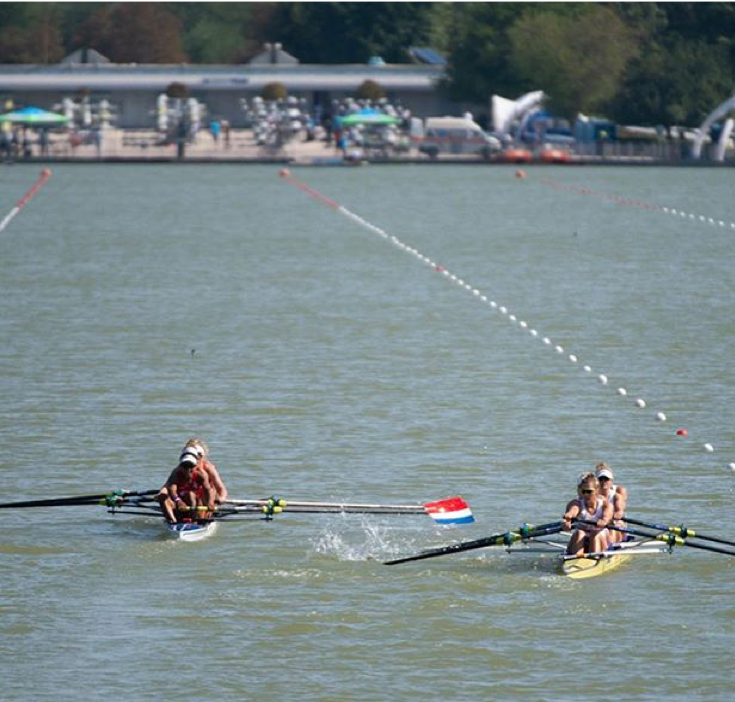
\includegraphics[width = \textwidth]{Images/w4steering.png} %this tells latex what graphics to include. I put my images in an 'Images' folder to aid file management, hence the Images/ before the file name. the width bit before allows you to alter the width of the image. It is also possible to use scale as well as using equations with the textwidth to make it say half the text width.
    \caption{GB W4- rowing behind the Dutch W4- during the 2018 World Championships \copyright Merijn Soeters} % this prints the caption below the figure
    \label{fig:four} % this internally labels the figure for future referencing.
\end{figure}

\LaTeX{} will helpfully(?) try to position the figure/table/image where it thinks it fits best into the text. You may disagree with \LaTeX{}, which is fine. To disagree there are many options. I tend to force \LaTeX{} to put the figure where I have put the figure environment in my code as this often allows me better control of the image positioning. This is done using [H] on the same line as the \verb+\begin{figure}+ command. There are other places you can force the figure to be placed and these are covered in \url{https://www.overleaf.com/learn/latex/Positioning_images_and_tables}. Please see the annotated code for this chapter for an example.

\section{Multiple Images}

It is also possible to put multiple images side by side to compare them. Please look at the code for the following images to see how this is done.

\begin{figure} [H]
\centering
\begin{subfigure}{.5\textwidth}
  \centering
  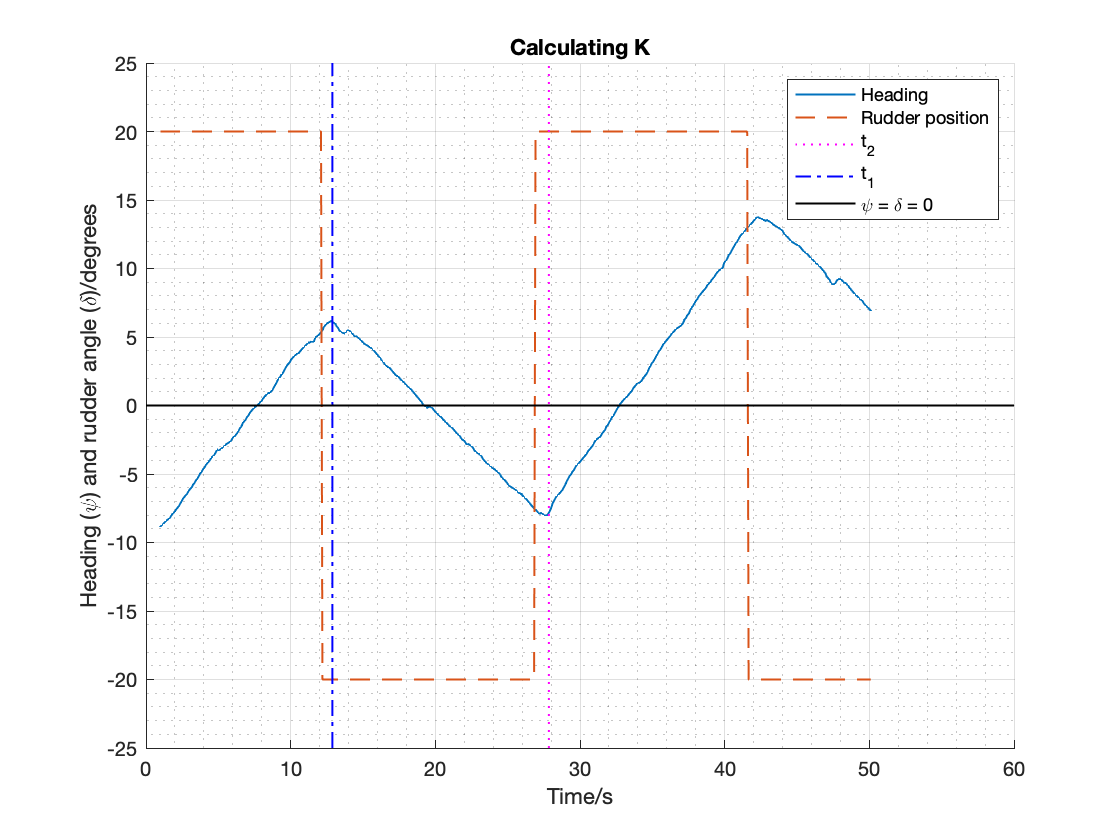
\includegraphics[width=1\linewidth]{Images/calculatingK.png}
  \caption{Derivation of K}
  \label{fig:KempfK}
\end{subfigure}
\begin{subfigure}{.5\textwidth}
  \centering
  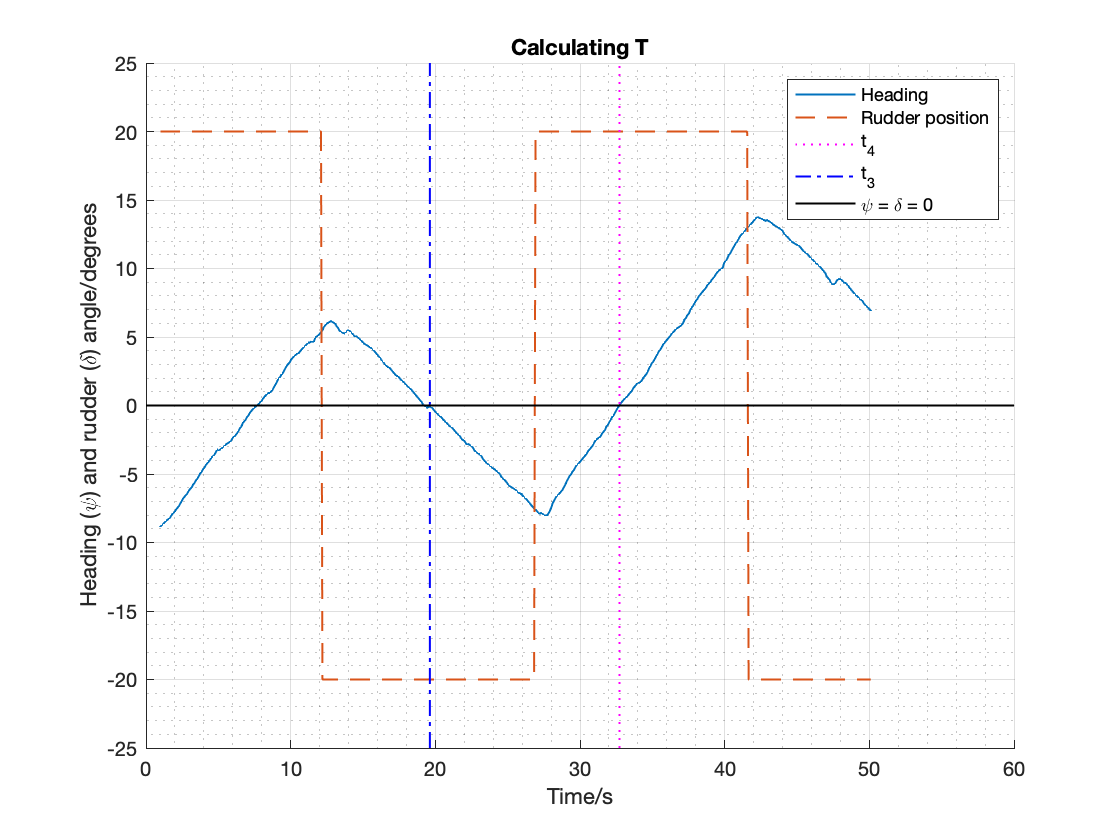
\includegraphics[width=1\linewidth]{Images/calculatingT.png}
  \caption{Derivation of T}
  \label{fig:KempfT}
\end{subfigure}
\caption{Results from Kempf maneuver}
\label{fig:kempf}
\end{figure}

\section{Drawing in \LaTeX{}}

It is also possible to draw diagrams in \LaTeX{}. Information on this can be found here \url{https://www.overleaf.com/learn/latex/Picture_environment}. (It is also possible to do many other things using \LaTeX{} as it is a Turing-complete programming language. However, if at any point in time you are tempted to use \LaTeX{} for anything other than typesetting, you should stop whatever you are doing and seek help from HUHS).

\section{Graphs in \LaTeX{}}

It is also possible to draw graphs in \LaTeX{}. These come out looking rather nice, and may be preferable to MATLAB graphs, though the extra hassle may negate any prettiness benefit. See \url{https://www.overleaf.com/learn/latex/Pgfplots_package} for details.